\documentclass[notes,11pt, aspectratio = 169]{beamer}
%
\usepackage[longnamesfirst,authoryear,sort,comma]{natbib}
\bibliographystyle{ecta}

\usepackage{bbding} % for \HandRight
\usepackage{slidespreamble}


\title{Local Projections and DiD}

\author{Christoph Hedtrich}

\date{\today}



\begin{document}

 
\begin{frame}
  \titlepage
\end{frame}

\begin{frame}\frametitle{When does Local Projection make sense in a panel?}
    \begin{wideitemize}
        \item \citet{jorda2005estimation} huge success in macro
            \begin{itemize}
                \item Goal: estimate impulse response functions in a single time-series 
                \item Approach: estimate a sequence of OLS regressions of $y_{t+h}$ on shock and controls in $t$ for $h = 0, 1, \dots, H$
            \end{itemize}
        \item DiD literature highlights issues with 
            \begin{itemize}
                \item Staggered Treatments 
                \item Heterogeneous Treatment Effects 
                \item Dynamic Treatment Effects 
                \item[$\rightarrow$] \href{https://github.com/paulgp/applied-methods-phd}{see Paul GP course}
            \end{itemize}
        \item \textcolor{red}{If DiD has all these issues, then LP must have them too!}
    
    \end{wideitemize}

\end{frame}



\begin{frame}\frametitle{\citet{de2022difference}}
    \begin{wideitemize}
        \item highlights issues with panel local projections 
            \begin{itemize}
                \item applied in complicated DiD treatment settings (continuous treatment intensity, staggered treatment, dynamic effects)
                \item "contamination by future"
                \item sign-reversal, even with positive treatment effects in every cell estimates may turn negative
                \item[$\rightarrow$] generalize event-study design  
            \end{itemize}
        \item General takeaway:TWFE+LP $\rightarrow$ misspecified regression when there is variation in treatment timing
      
    \end{wideitemize}

\end{frame}


\begin{frame}\frametitle{\citet{dube2023local} \href{https://conference.nber.org/conf_papers/f172417.slides.pdf}{Slides}}

    \begin{wideitemize}
        \item \textbf{Goal:} estimate treatment effects in a panel with typical DiD issues
        \item \textbf{Solution:} select observations appropriately/control for previous treatments 
        \item LP is just OLS, so this is super fast compared to other suggested estimators           
    \end{wideitemize}
\end{frame}


\begin{frame}
    \frametitle{Which issues from DiD literature carry over to LP setting with shocks?}
        \begin{wideitemize}
            \item Staggered Treatment $\rightarrow$ What happens with trend in treatment intensity? 
            \item Heterogeneous Treatment Effects $\rightarrow$ Bias even with mean zero shocks? 
            \item Dynamic Treatment Effects 
        \end{wideitemize}

\end{frame}

\begin{frame}\frametitle{IRF in panel with TWFE +LP}
    \[ y_{it} = \alpha_i + \phi_t + \beta_{0,i} s_{it} +\rho_i y_{it-1} +\varepsilon_{it} , \] 
    \begin{wideitemize} 
\item where 
    \begin{itemize}
        \item groups  $i =1 , \dots, I$ 
        \item time periods $t = 1, \dots, T$ 
        \item outcome of interest $y_{it}$
        \item shock  $s_{it}$ (continuous shock)
        \item group specific intercept $\alpha_i$ and trend $g_{it}$
        \item time specific intercept $\phi_t$ 
        \item $\varepsilon_{it} \sim N(0, \sigma^2)$ i.i.d. 
    \end{itemize}
    \item  Treatment Effects/IRF:        \[\beta_h = \beta_{0,i} \rho_i^{h-1} \quad \forall h\geq0  \] 
  
\end{wideitemize}

\end{frame}


\begin{frame}\frametitle{IRF in panel with TWFE +LP}

    \begin{wideitemize} 
        \item Simulate with  
        \begin{enumerate}
            \item group specific shock mean $s_{it} \sim N(\mu_i, \sigma_s^2)$
            \item time specific shock mean $s_{it} \sim N(\mu_t, \sigma_s^2)$
            \item Heterogeneous treatment effects $\beta_{0,i}$ 
            \item trend in shock mean $\mu_{i,t} = \mu_i + \gamma_i t$ 
        \end{enumerate}
        \item Monte Carlo: 
            \begin{itemize}
                \item $10 000$ repititions 
                \item $I = 2$ groups
                \item $T = 100$ time periods
                \item common AR process $\rho_i=\rho$
            \end{itemize}
    \end{wideitemize}

\end{frame}

  

\begin{frame}
    \frametitle{Case 1: Group specific shock mean}
    \[E[s|i] \neq E[s|i'] \] 
    
    
\begin{figure}
    \centering
    \subfloat[$h=0$]{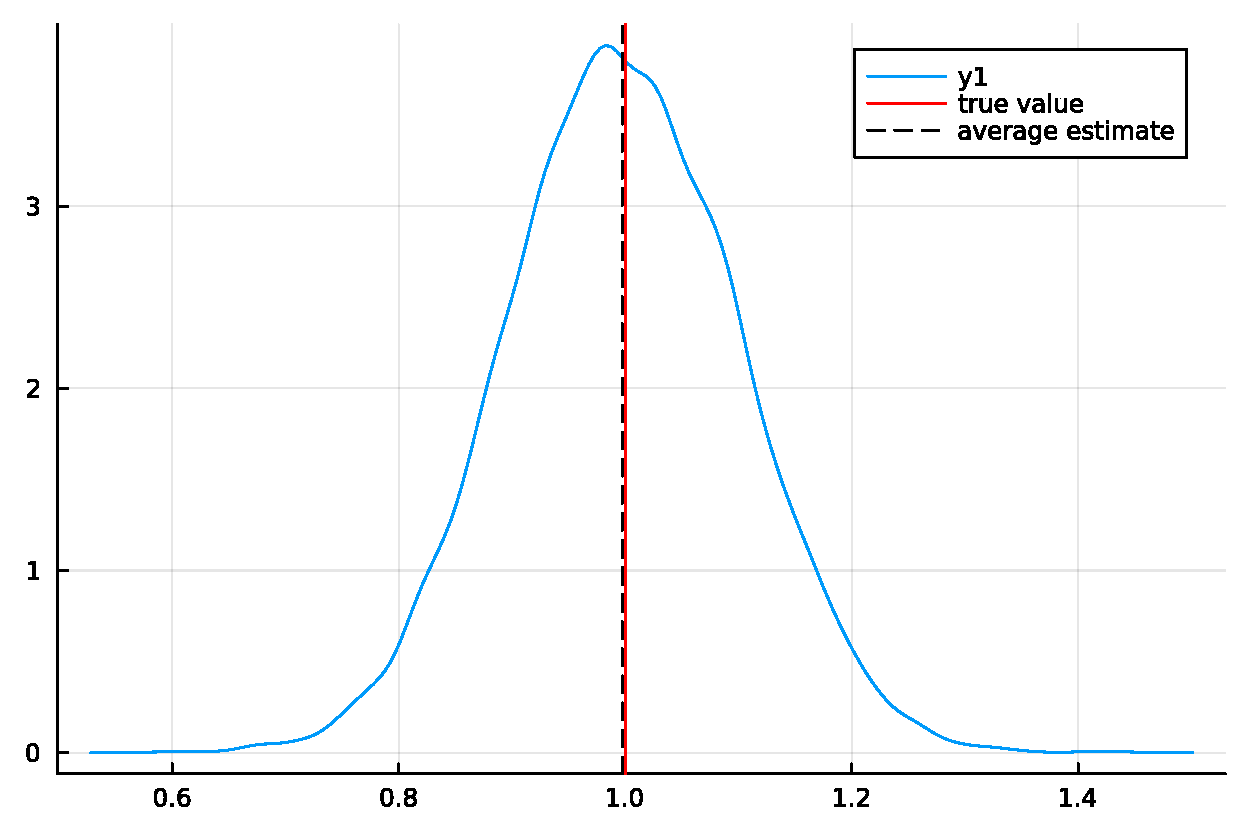
\includegraphics[width=0.3\textwidth]{./img/bh0case1.pdf}}
    \subfloat[$h=1$]{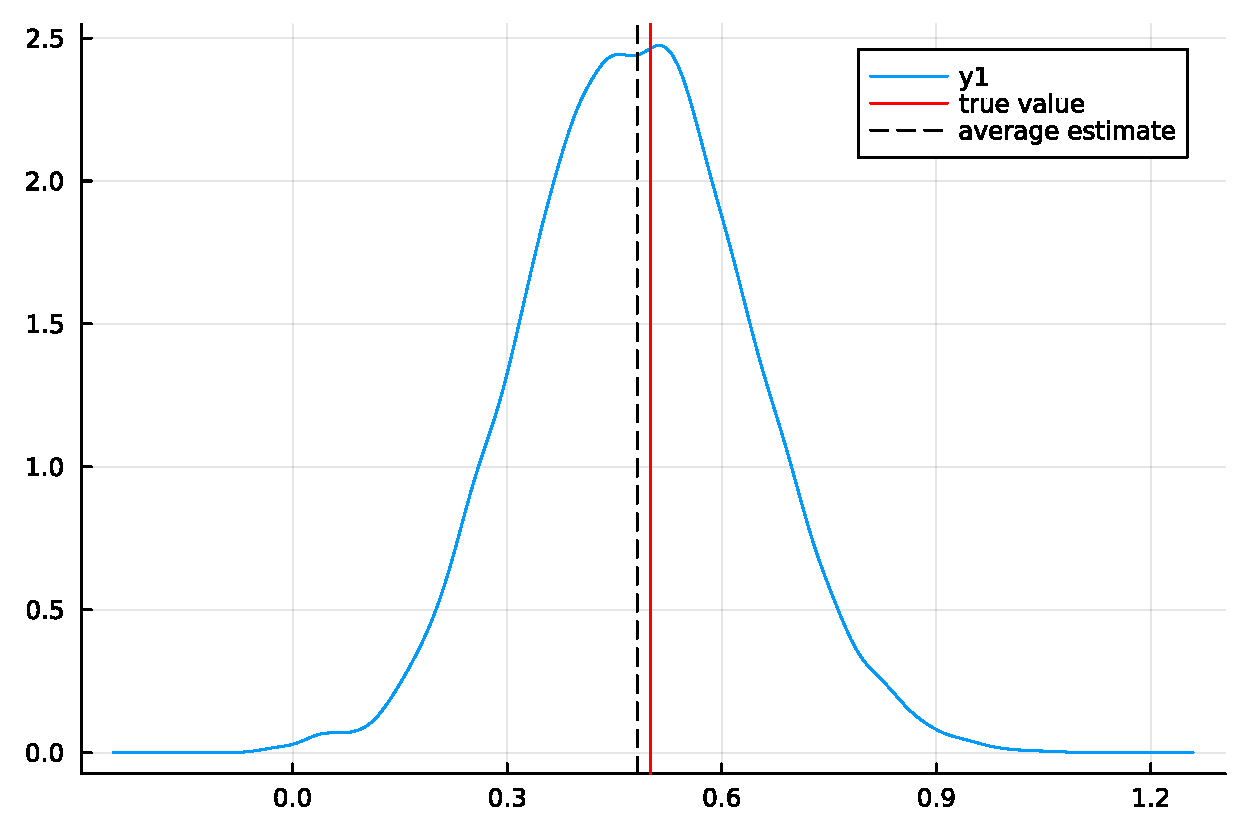
\includegraphics[width=0.3\textwidth]{./img/bh1case1.pdf}}
    \subfloat[$h=2$]{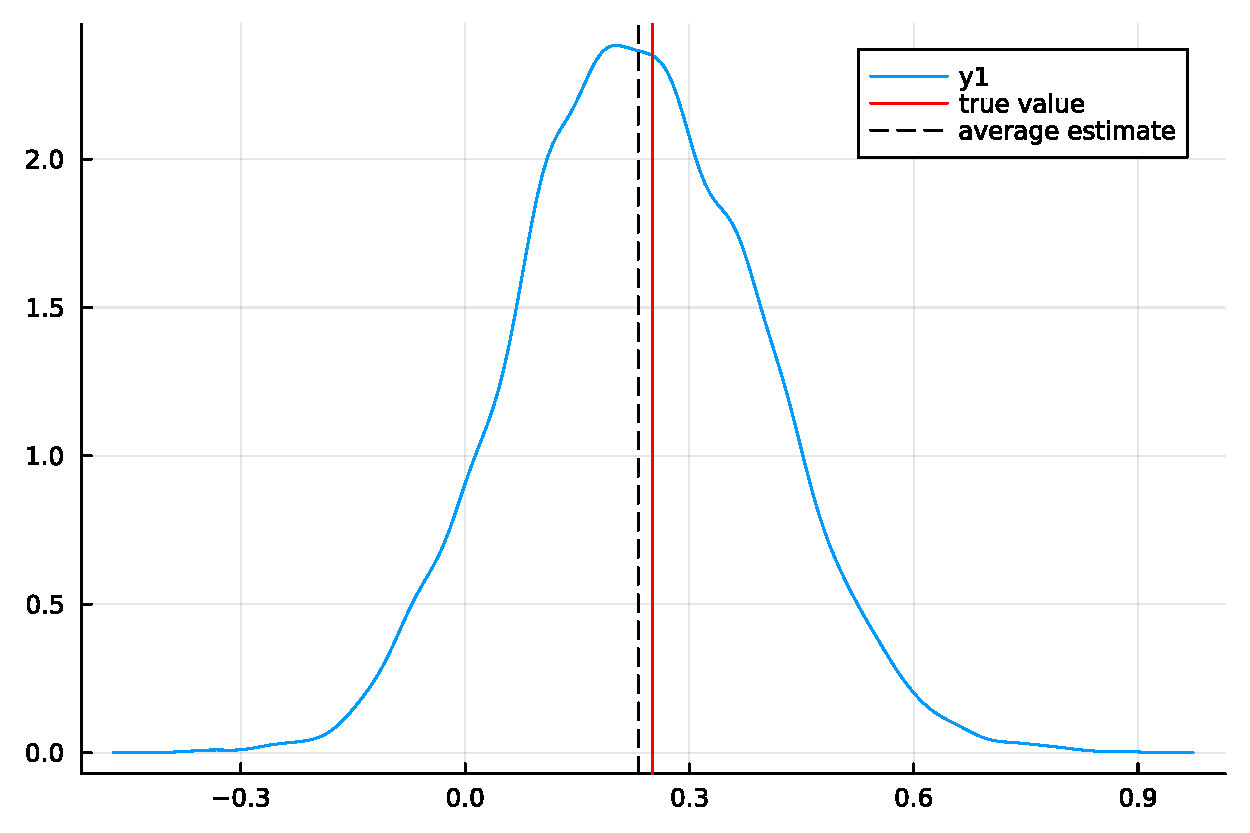
\includegraphics[width=0.3\textwidth]{./img/bh2case1.pdf}}
  \caption{IRF Case 1}
  \end{figure}
  
  No problem with group specific shock mean (as expected)
  
\end{frame}


\begin{frame}\frametitle{Case 2: Time specific shock mean (common across groups)}
    \[E[s|t]=E[s|t,i]=g t \] 
    
    \begin{figure}
        \centering
        \subfloat[$h=0$]{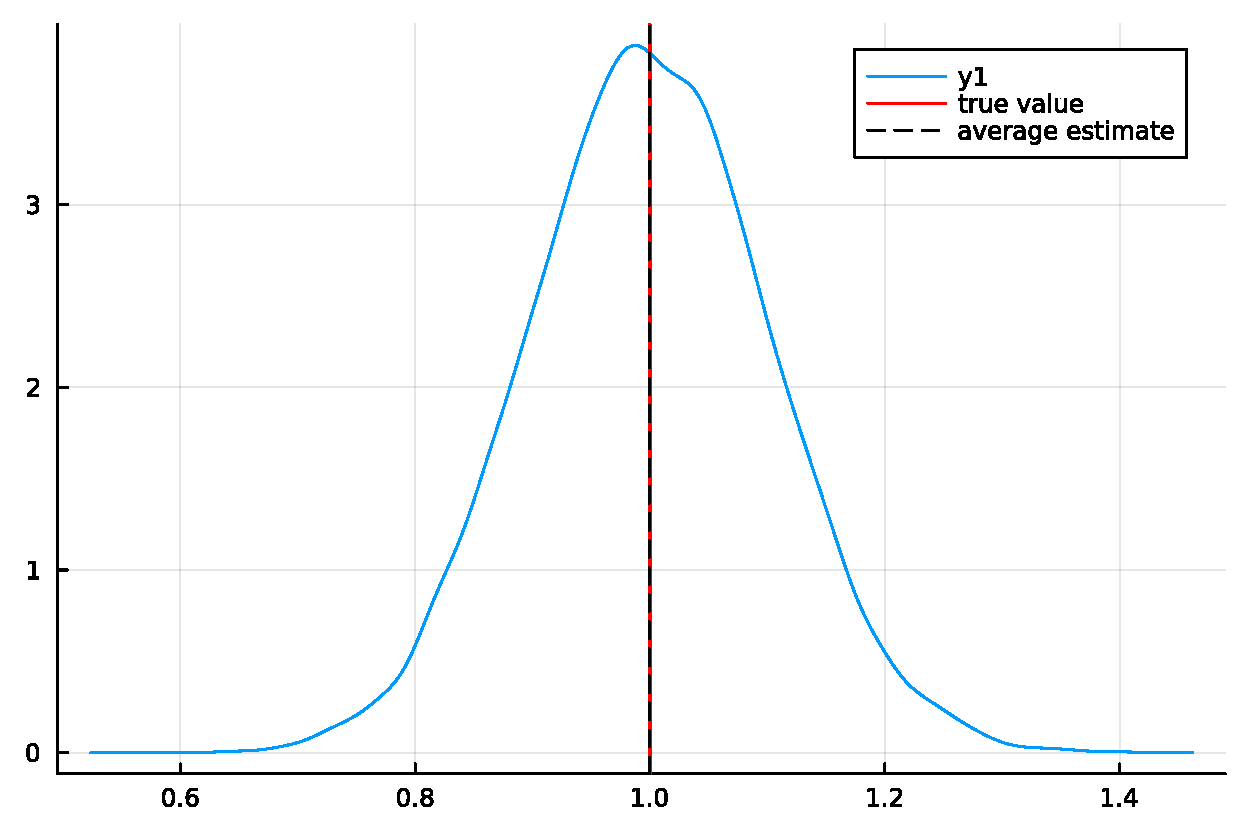
\includegraphics[width=0.3\textwidth]{./img/bh0case2.pdf}}
        \subfloat[$h=1$]{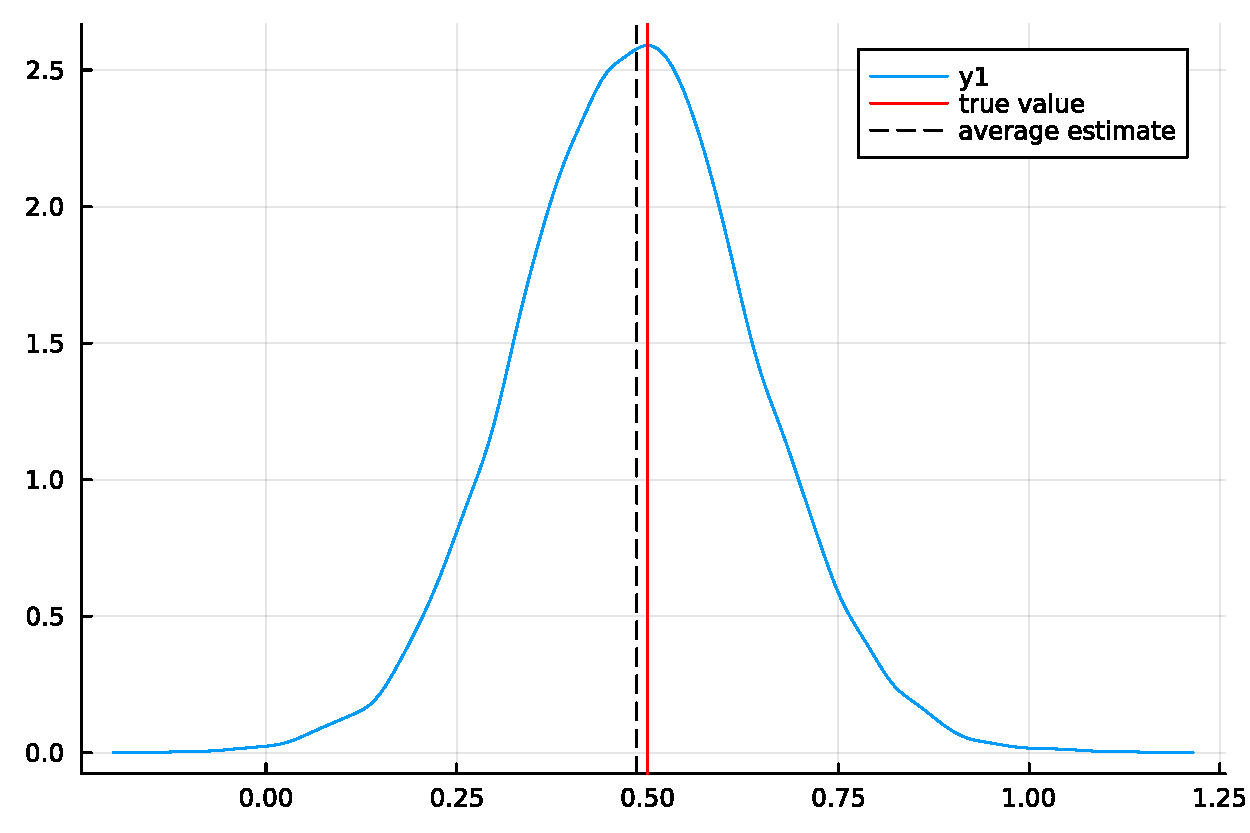
\includegraphics[width=0.3\textwidth]{./img/bh1case2.pdf}}
        \subfloat[$h=2$]{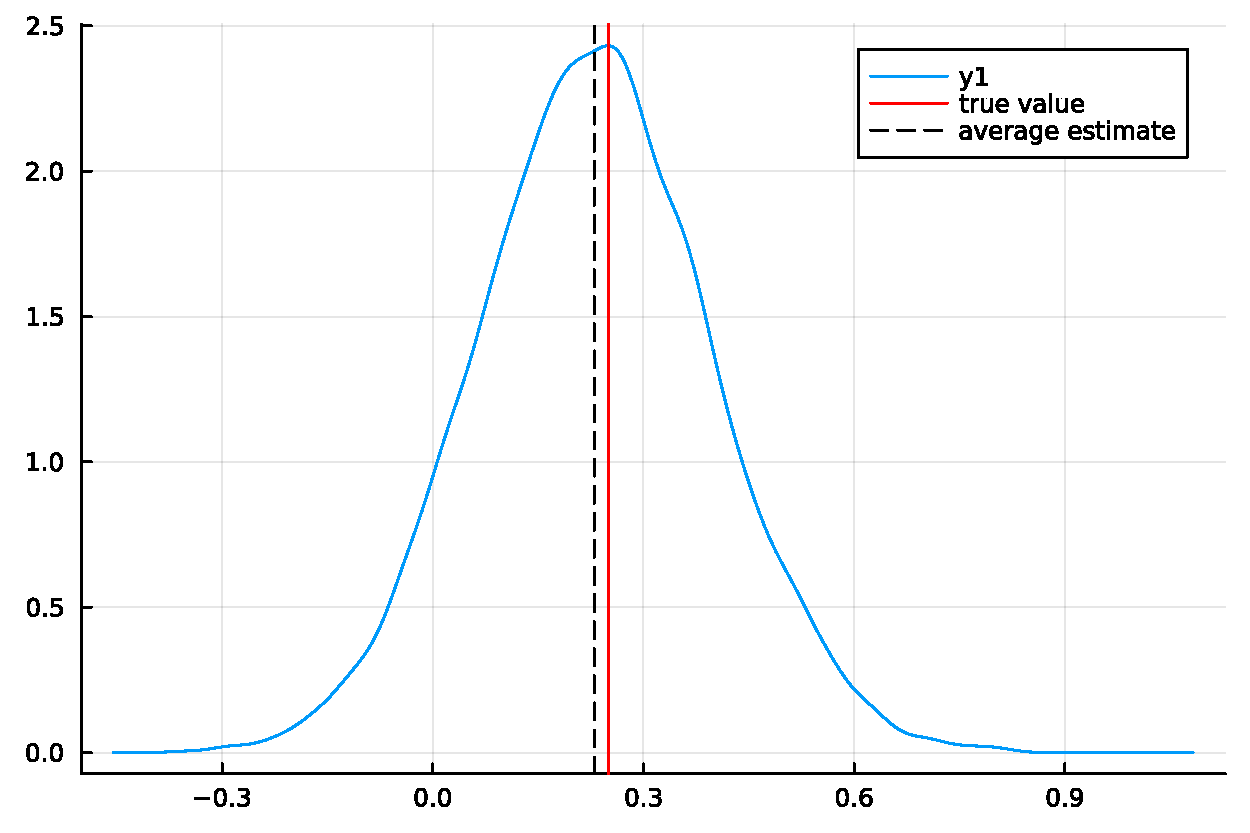
\includegraphics[width=0.3\textwidth]{./img/bh2case2.pdf}}
      \caption{IRF Case 2}
      \end{figure}
      
      No problem with time specific shock mean (as expected)
    

\end{frame}

\begin{frame}\frametitle{Case 3: Does TWFE+LP estimate "average treatment effect" with heterogeneous treatment effects?}
    \[\beta_{0,i} \neq \beta_{0,i'}\] 

    \begin{figure}
        \centering
        \subfloat[$h=0$]{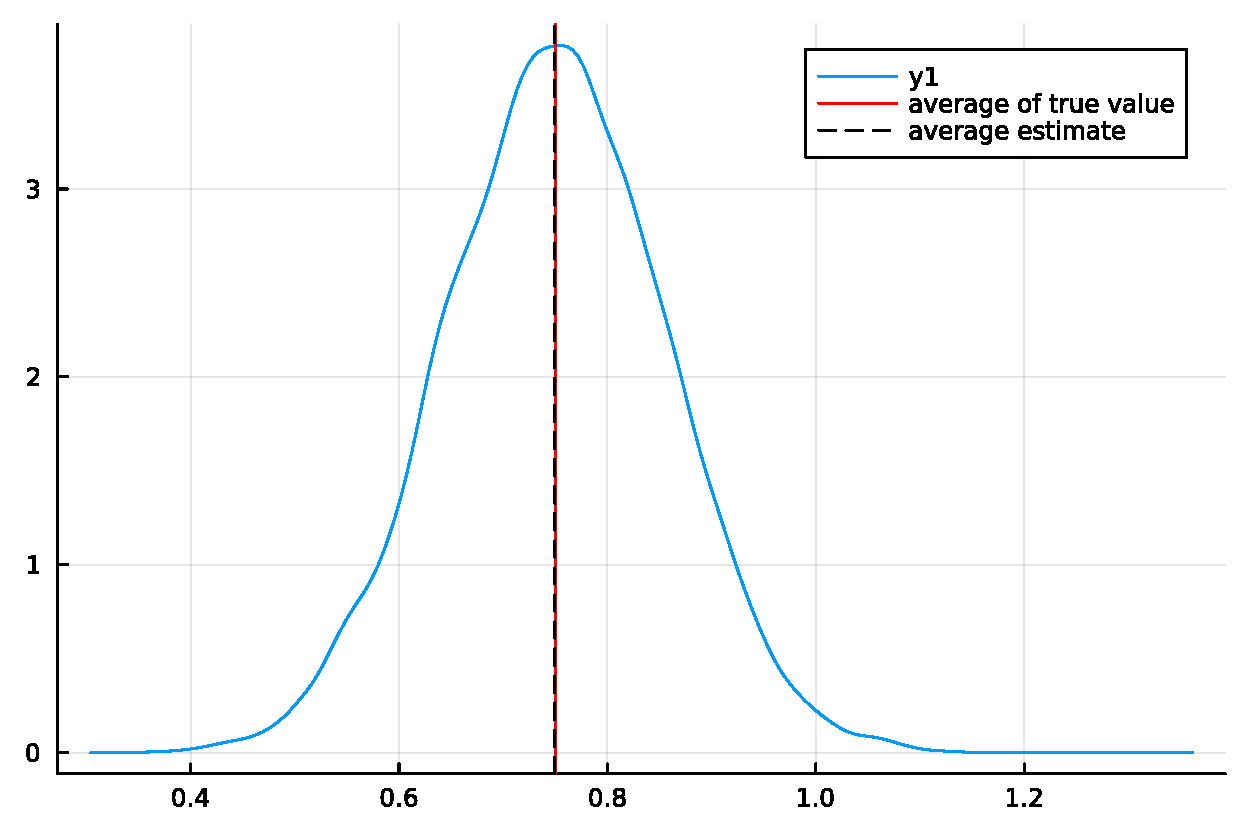
\includegraphics[width=0.3\textwidth]{./img/bh0case3.pdf}}
        \subfloat[$h=1$]{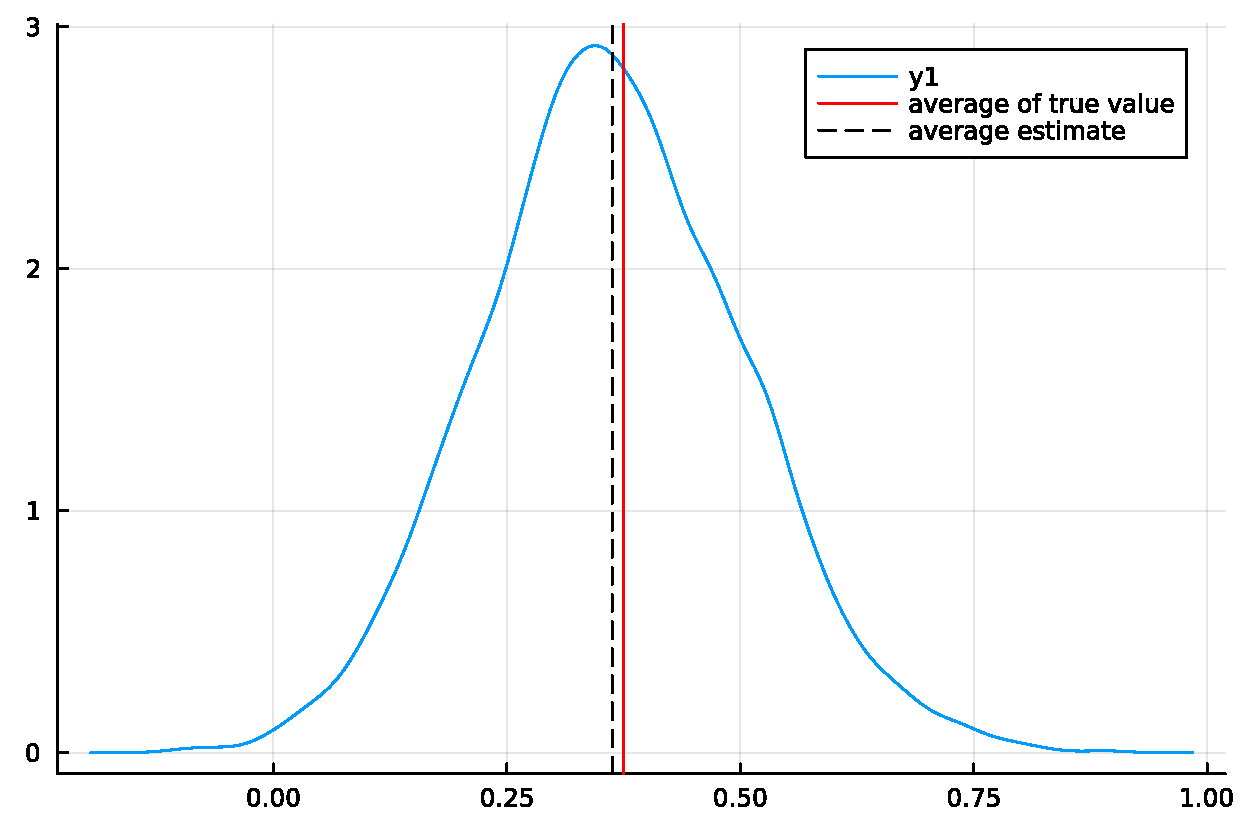
\includegraphics[width=0.3\textwidth]{./img/bh1case3.pdf}}
        \subfloat[$h=2$]{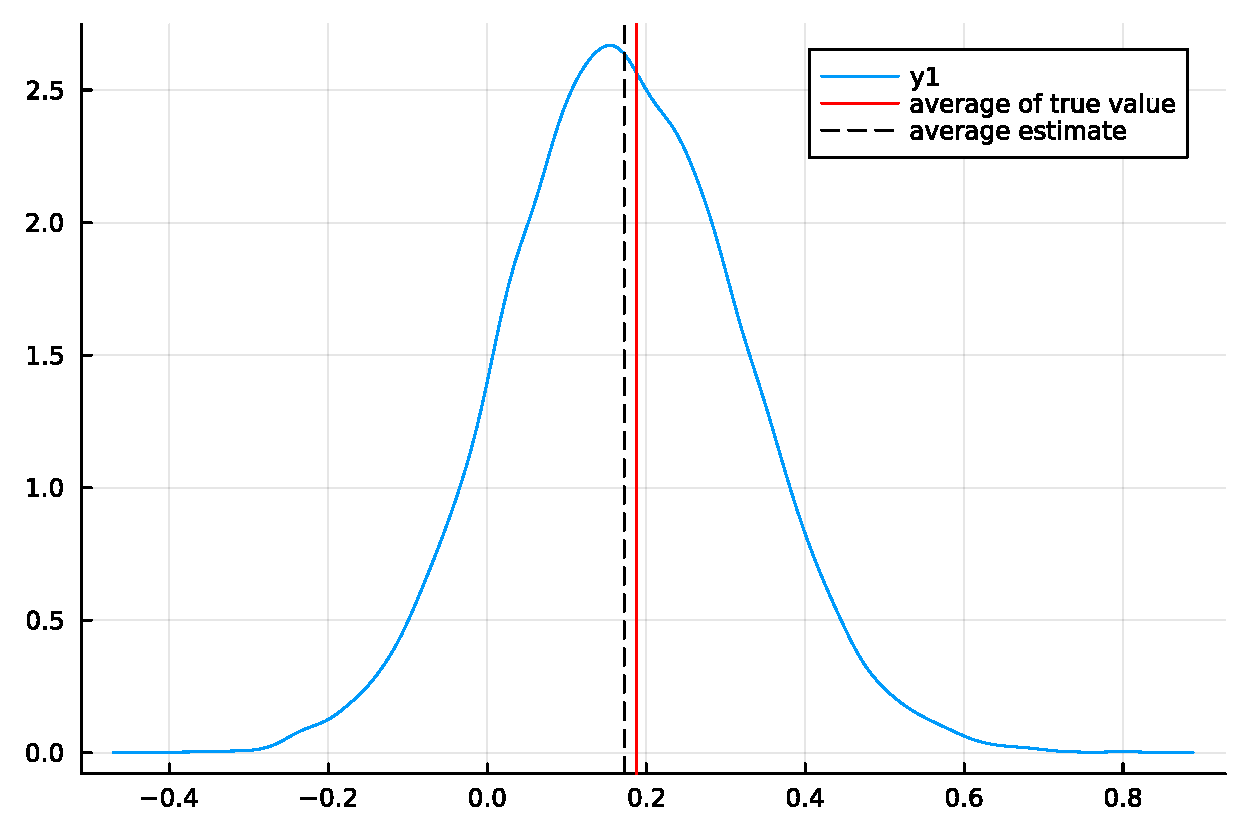
\includegraphics[width=0.3\textwidth]{./img/bh2case3.pdf}}
      \caption{IRF Case 3}
      \end{figure}
      
      No problem with heterogeneous treatment effects by itself

\end{frame}


\begin{frame}\frametitle{Case 4 a): Trend in treament intensity by group }
    \begin{wideitemize}
        \item TWFE-DiD had issues with staggered treatment  $\rightarrow$ trend in treatment intensity by group  
            \[E[s|t,i] = g_i t\] 
        \item[$\rightarrow$] IRF is biased for $h>0$ 
    \end{wideitemize}

    \begin{figure}
        \centering
        \subfloat[$h=0$]{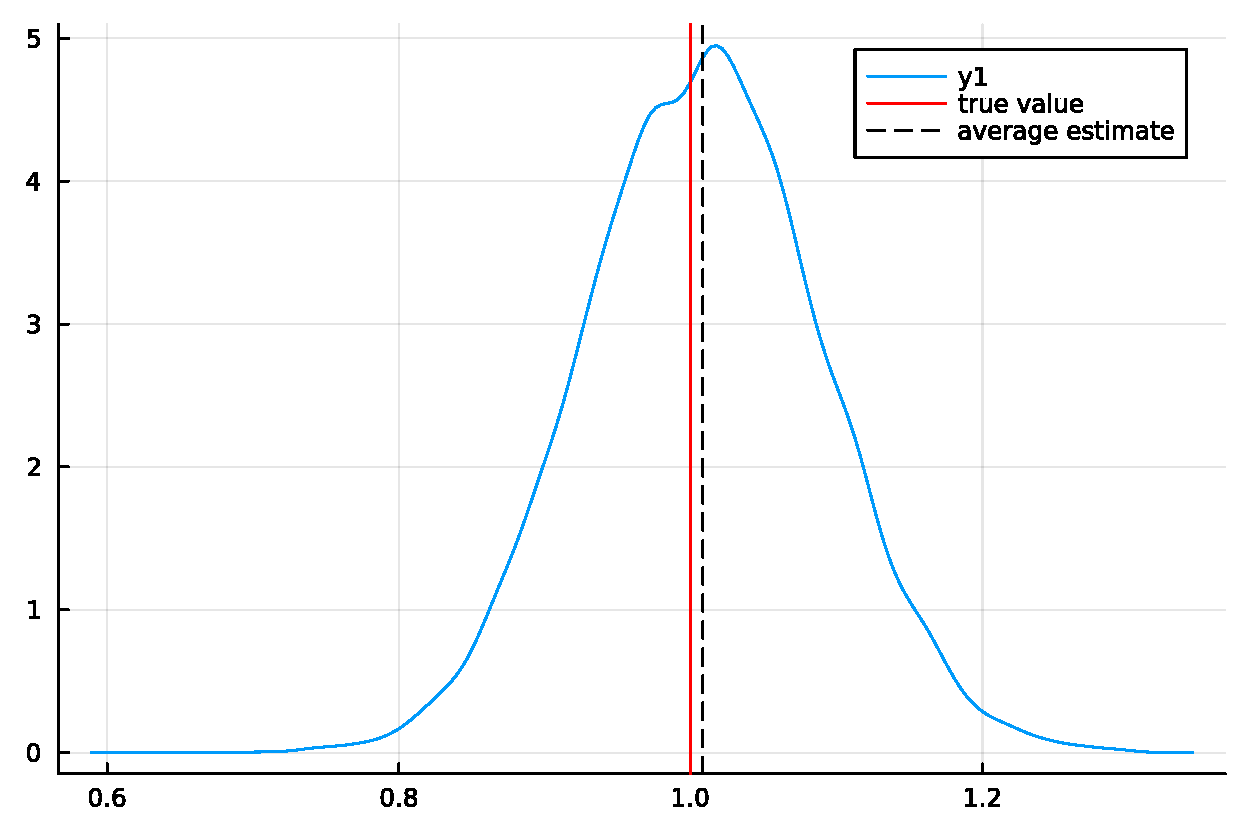
\includegraphics[width=0.3\textwidth]{./img/bh0case4a.pdf}}
        \subfloat[$h=1$]{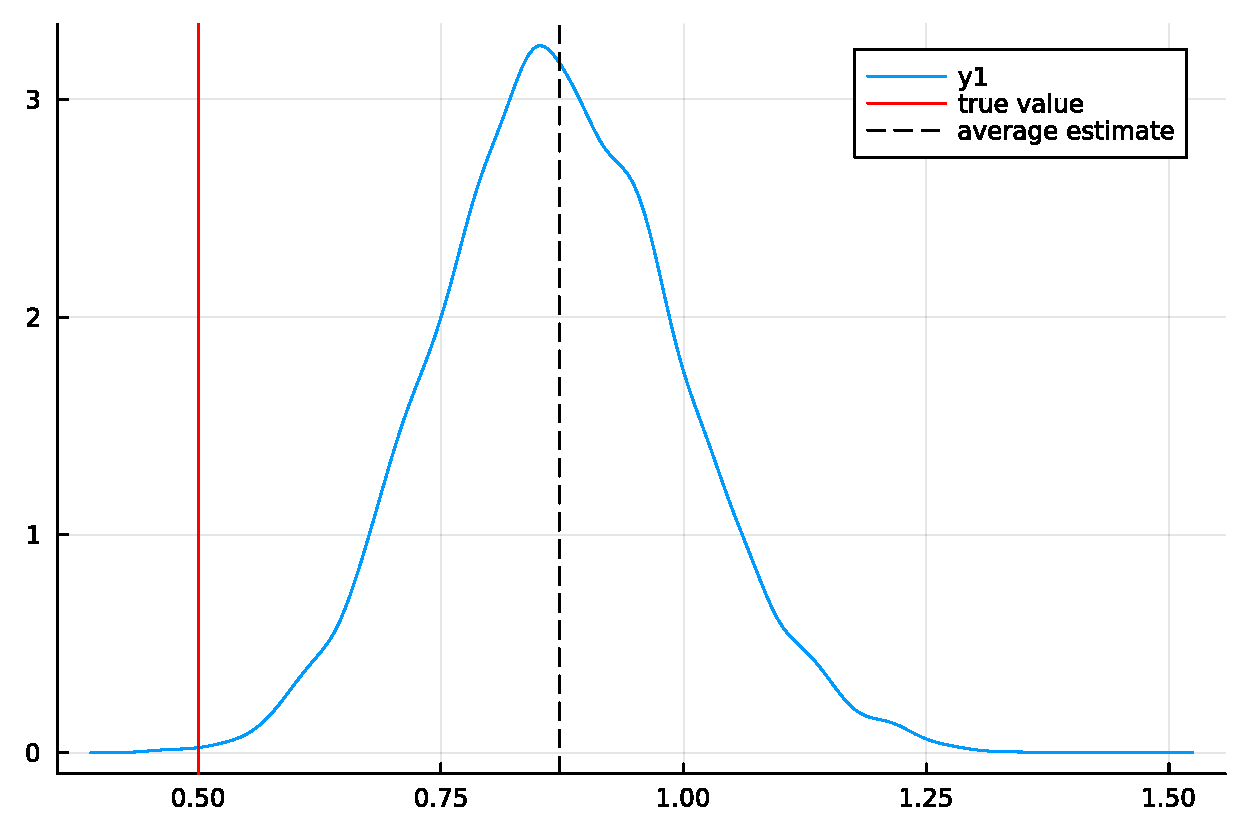
\includegraphics[width=0.3\textwidth]{./img/bh1case4a.pdf}}
        \subfloat[$h=2$]{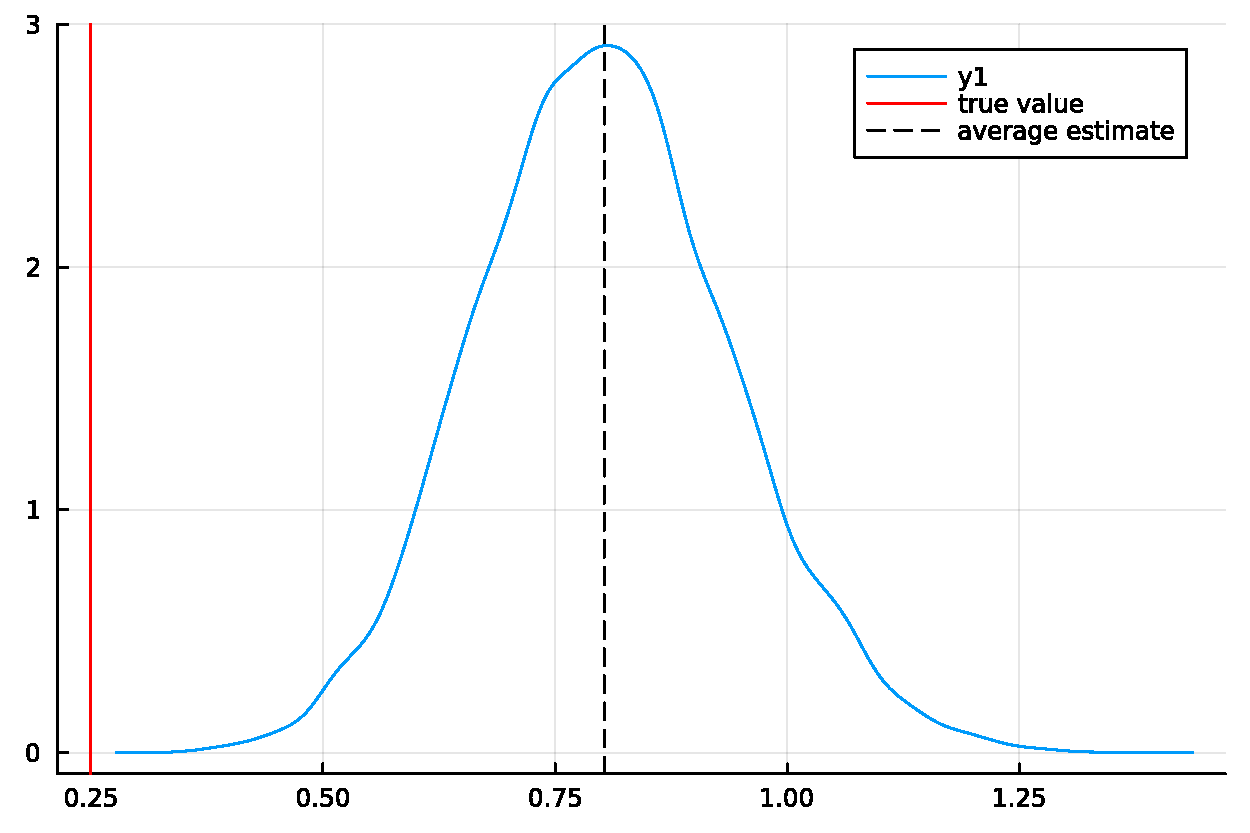
\includegraphics[width=0.3\textwidth]{./img/bh2case4a.pdf}}
      \caption{IRF Case 4 a}
      \end{figure}
\end{frame}


\begin{frame}\frametitle{Case 4 b): Trend in treament intensity by group + Heterogeneous Treatment Effects }
    \begin{wideitemize}
        \item TWFE-DiD had issues with staggered treatment + heterogeneous treatment effects
        \item Analogue: trend in treatment intensity by group  + heterogeneous treatment effects
    \end{wideitemize}

    \begin{figure}
        \centering
        \subfloat[$h=0$]{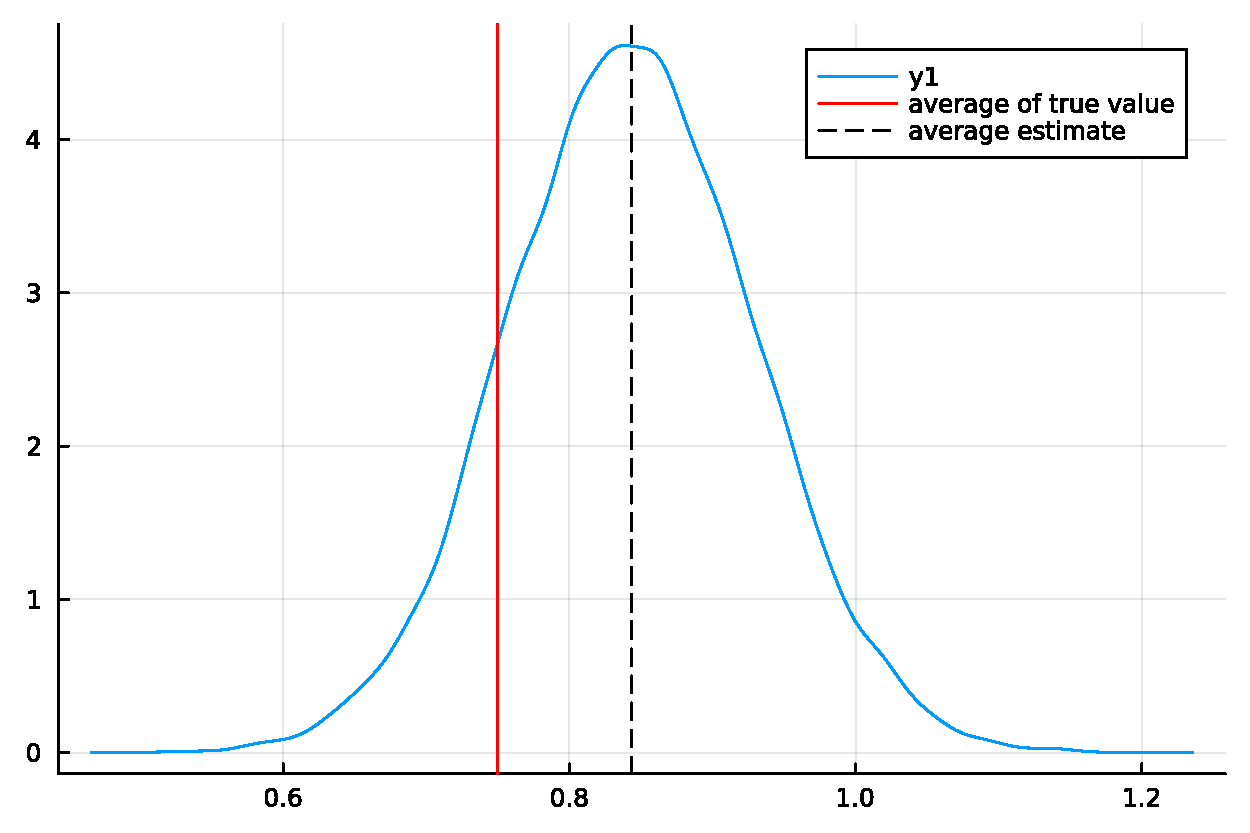
\includegraphics[width=0.3\textwidth]{./img/bh0case4b.pdf}}
        \subfloat[$h=1$]{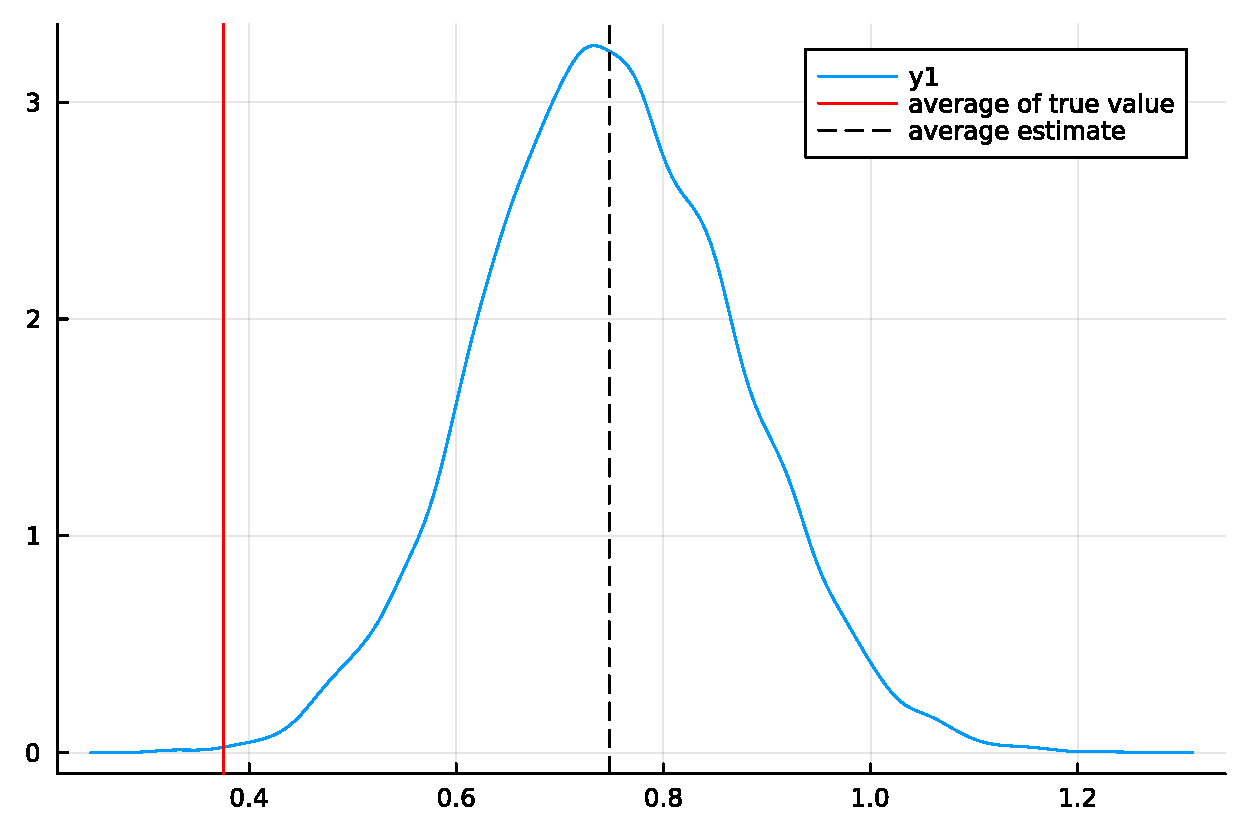
\includegraphics[width=0.3\textwidth]{./img/bh1case4b.pdf}}
        \subfloat[$h=2$]{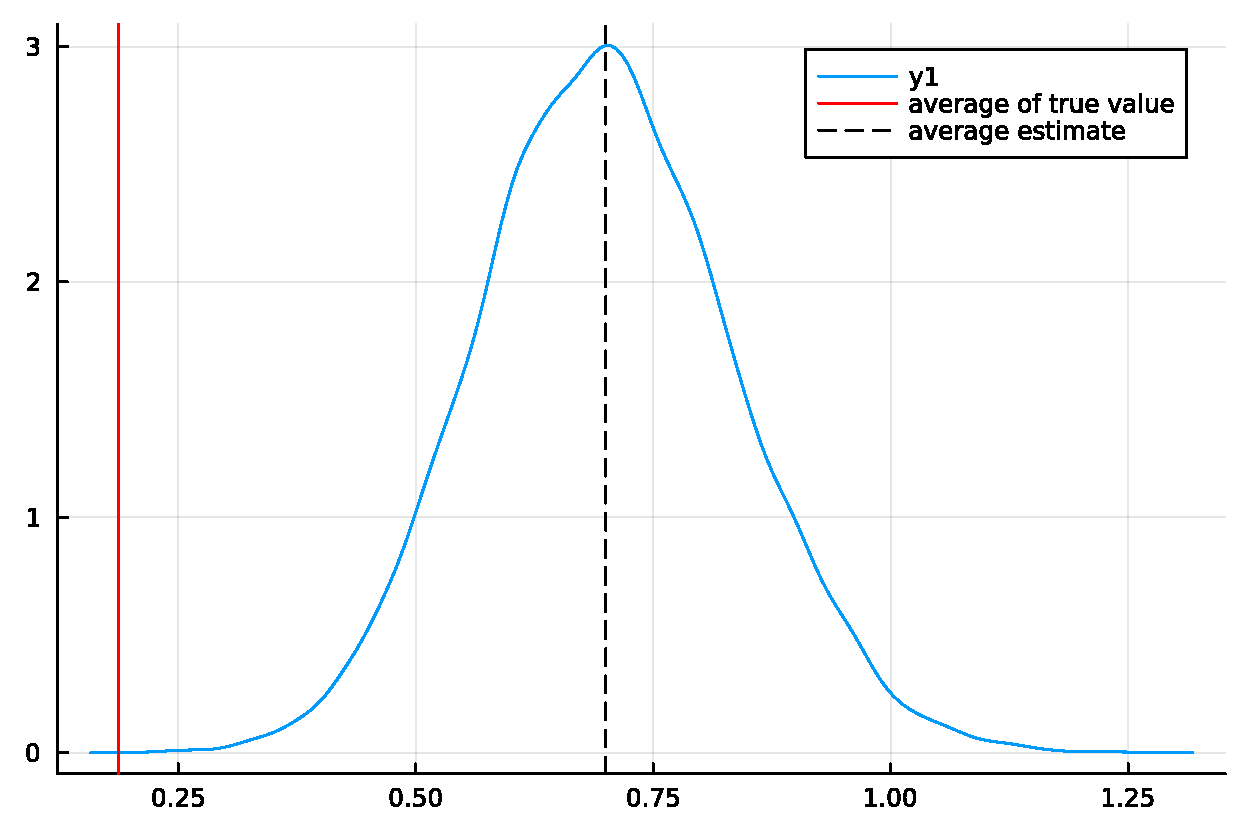
\includegraphics[width=0.3\textwidth]{./img/bh2case4b.pdf}}
      \caption{IRF Case 4 b}
      \end{figure}
\end{frame}


\begin{frame}\frametitle{Case 4 b): Trend in treament intensity by group + Heterogeneous Treatment Effects (ctd.)}
    \begin{wideitemize}
        \item Add a group specific trend:
         \[ y_{it} = \alpha_i + \phi_t + \beta_{0,i} s_{it} +\rho_i y_{it-1} + g_{i}t +\varepsilon_{it} , \]  
    \end{wideitemize}

    \begin{figure}
        \centering
        \subfloat[$h=0$]{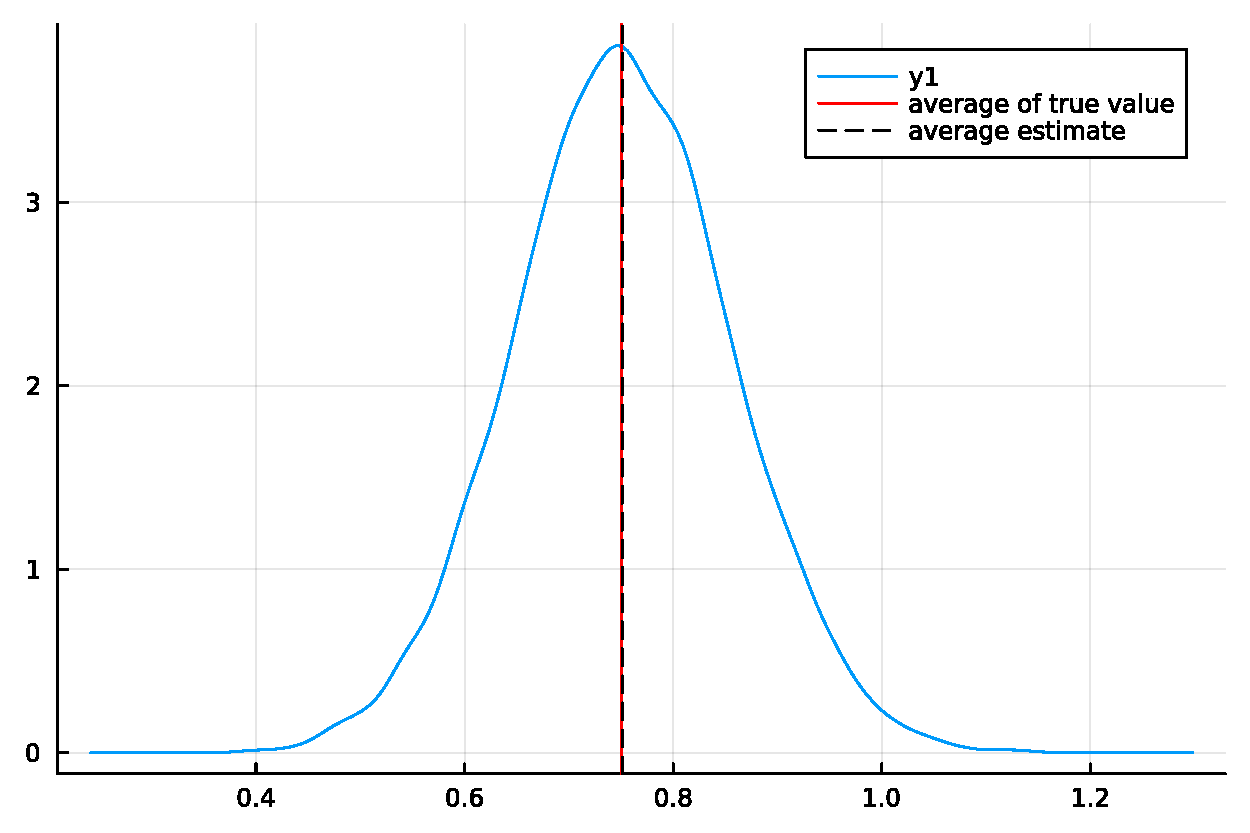
\includegraphics[width=0.3\textwidth]{./img/bh0case4b_trend.pdf}}
        \subfloat[$h=1$]{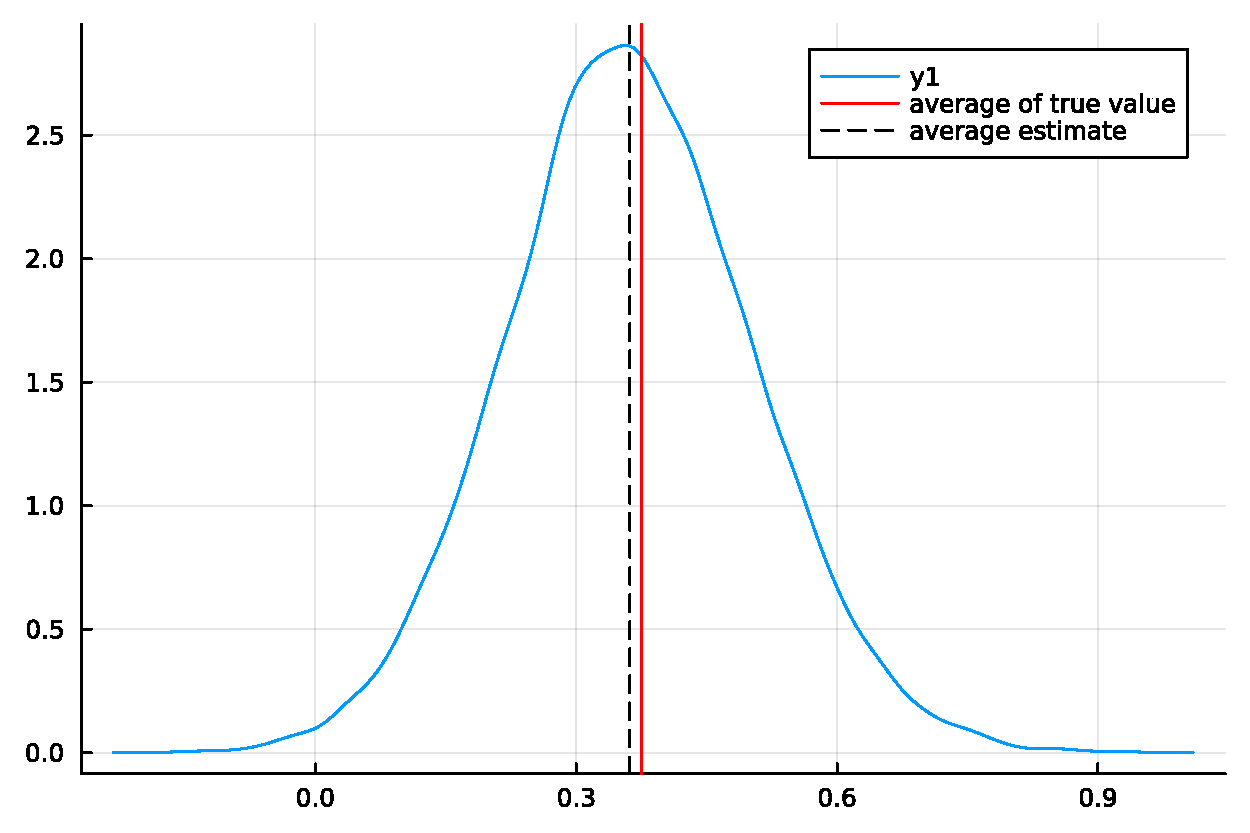
\includegraphics[width=0.3\textwidth]{./img/bh1case4b_trend.pdf}}
        \subfloat[$h=2$]{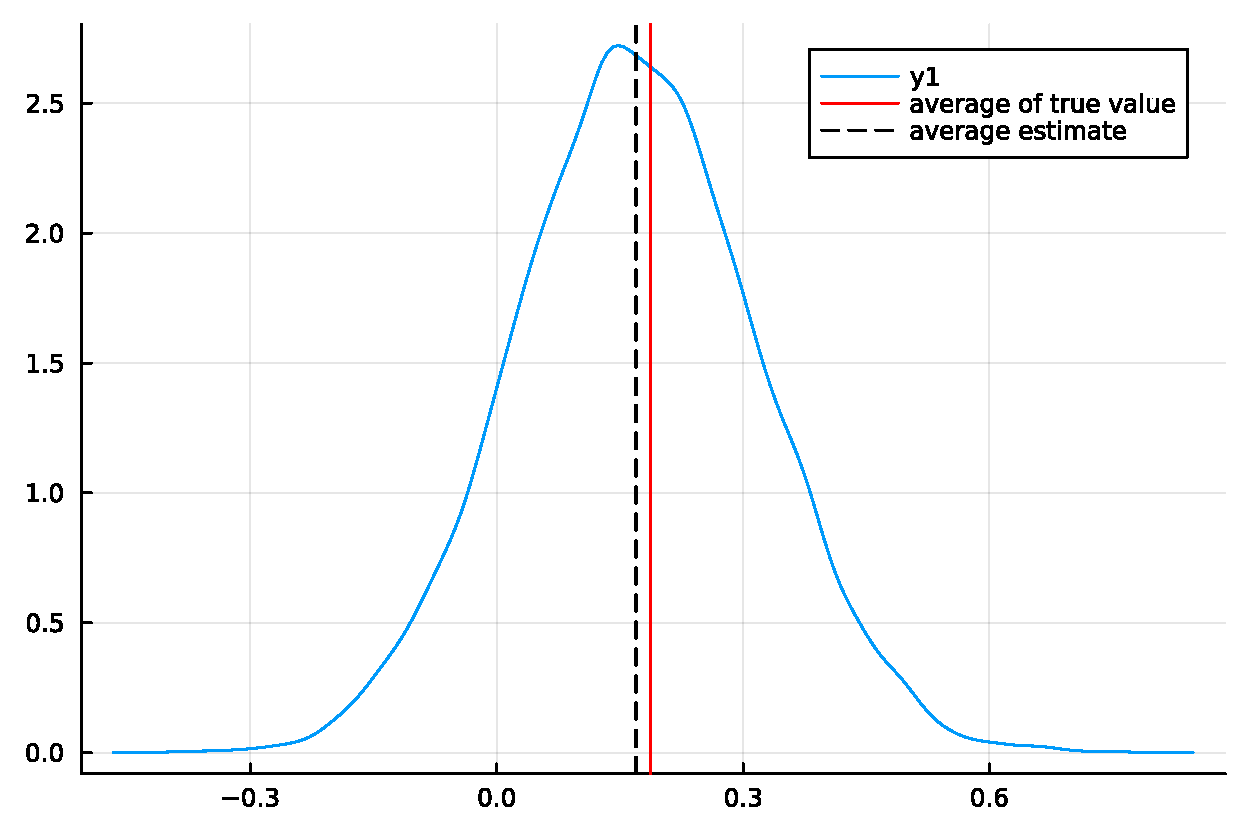
\includegraphics[width=0.3\textwidth]{./img/bh2case4b_trend.pdf}}
      \caption{IRF Case 4 b with linear trend by group}
      \end{figure}
\end{frame}






\begin{frame}\frametitle{Local Projection in Panel}
   See \url{git@github.com:chrished/localprojection_panel.git} for simulation code
    \begin{wideitemize}
        \item[1] Case with few treatment times, see \cite{dube2023local} and literature in \href{https://github.com/paulgp/applied-methods-phd}{Paul GP course}
        \item[2] Continuous shocks in (almost) every period: 
        \begin{itemize}
            \item group specific trend in treament intensity $\rightarrow$ Biased estimates for $h>0$ (similar to staggered treatment) 
            \item heterogeneous treatment effects  $\rightarrow$ Biased estimates $\forall h$
            \item[$\rightarrow$] Need to control for group specific trends! 
        \end{itemize}
        \item What is the correct way? \citet{de2022difference}? 
        \item Is it okay to simply "de-trend" shocks? 
        \item Other issues that would bias estimates?
        \item Inference? (small sample estimates of $\alpha_i$ and $\phi_t$, serial correlation, ... )
    \end{wideitemize}

\end{frame}

\begin{frame}[allowframebreaks]{References}

    \bibliography{./refs}
    
    \end{frame}

\end{document}